\chapter {Arquitetura}

Como ambiente de desenvolvimento integrado (IDE) escolhido foi o eclipse devido ao favorecimento do desenvolvimento rápido com recursos que podem ser integrados através de plugins, além disso sua portabilidade para outras plataformas sem afetar os plugins adicionados favorecendo o desenvolvimento independente da plataforma escolhida pelo desenvolvedor.\\

O Eclipse Java development tools (JDT), fornece plugins que implementam a IDE eclipse servindo com apoio para o desenvolvimento de qualquer aplicativo Java, inclusive plugins para a própria IDE Eclipse.\\

São cinco os componentes que compõem o JDT, e cada componente pode operar com um projeto independente, que são:

	\begin{itemize}
		\item \textbf{APT} fornece plugins que adicionam e fornecem suporte ao processamento de anotações java.
		\item \textbf{Core} é o core da infraestrutura Java da IDE eclipse provendo compiladores, API's modelos definidas em árvores Java, documentação, assitente de código, suporte e formatação de código fonte.
		\item \textbf{Debug} componente de depuração da plataforma sendo definido independente da linguagem utilizada.
		\item \textbf{Text} fornece blocos básicos para editores de texto e textos dentro do eclipse e ainda contribui com o editor de texto padrão do eclipse. \item \textbf{UI} prove toda interface que necessite de iteração com o usuário final, e ainda fornece a manipulação e visualização do código Java na IDE.
	\end{itemize} 
	
\section {Arquitetura}

A arquitetura do analisador a ser implementada utiliza com base os componentes JDT porém de maneira independente da IDE eclipse o qual não é um plugin da IDE mas sim uma ferramente que pode ser utilizada como apoio em qualquer processo de desenvolvimento ou para levantamento de dados sobre a história evolutiva de um software.\\

Esta analisador tem com base para seu funcionamento o uso de visitors\cite{Gamma:1995:DPE:186897} os quais possuem inteligência para verificar a adoção de códigos recentemente adicionados a novas releases da linguagem Java como multicatchs e até mesmo efetuar a pesquisa de código ultrapassados através de padrões pré-definidos para que possam vir a ser melhorados caso o desenvolvedor assim julgue necessário conforme é o caso de vários catchs aninhados que pode ser um potencial caso de se tornar um bloco único de multicatch tornando o código mais elegante, atual e legível.\\

Tais analisador tem como entradas válidas um único arquivo arquivo separado por vírgula (CSV) que possui em seus campos o nome dos projeto, versões e caminho para que cada um seja analisado. Após o input é realizado uma pesquisa em seu diretório \textit{src} o qual contém os códigos Java que compõem o projeto, após todos os arquivos listas é realizado um parse para a construção de árvores de sintáxe abstratas (AST) uma por arquivo e dai é lançando os visitors\cite{Gamma:1995:DPE:186897} com suas respectivas inteligências para pesquisar os padrões previamente definidos os quais são armazenados em uma única coleção de dados que gera um CSV para cada padrão designado e dentro informando onde e em qual versão do projeto fora encontrado.\\
	
\begin{figure}[h]
	\center
	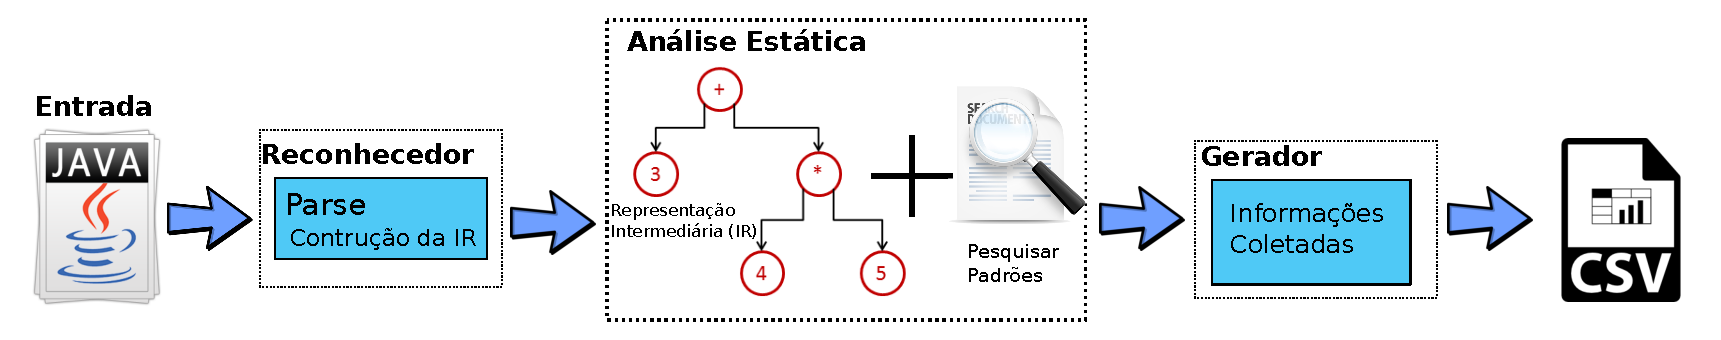
\includegraphics[width=1.0\textwidth]{Imagens/Arquitetura}
	\label{arquiteturaVisitor}
	\caption{Arquitetura geral do software.}
\end{figure}	

\clearpage
\subsection{Visitors}
\begin{figure}[h]
\center
\includegraphics[width=1.0\textwidth]{Imagens/Visitors}
\label{arquiteturaVisitor}
\caption{Organização dos Visitors.}
\end{figure}

Todos os visitors criados para o projeto extendem da classe \textit{Visitor.java} a qual implementa a interface \textit{IVisitor.java}, vale resaltar que a classe \textit{Visitor.java} extende por sua vez de ASTVisitor a qual é fornecida pelo Core do JDT eclipse tendo como método principal utilizado neste projeto o \textbf{boolean visit(Statement node)} o qual recebe como parâmento qualquer Statement descrito na lib JDT, este método é sobrescrito com todo conteúdo necessário para recolher as méticas de acordo com os padrões previamente estabelecidos.\\


\clearpage
\begin{figure}[h]
	\center
	\includegraphics[width=0.8\textwidth]{Imagens/ProjectAnalyser}
	\label{ProjectAnalyser}
	\caption{Project analyser.}
\end{figure}

Este diagrama exibe o coração da aplicação pois é aqui que ocorre a transformação de todo código Java que compõe o projete em árvore sintática para que os visitors\cite{Gamma:1995:DPE:186897} possam pesquisar em seus nós pelos padrões estabelecidos.\\

Um ponto interessante é que o \textit{ProjectAnalyser.java} não tem a responsabilidade de instanciar a lista de IVisitor a qual possui referência pois estas são injetadas usando o padrão de projeto injeção de dependência\textbf{(DI)} o qual aqui faz-se presente através do framework spring que injeta uma lista de \textit{bean} onde cada \textit{bean} representa cada classe de extendida de Visitor descrita anteriormente.\\

\clearpage


\subsection{Inversão de Controle e Injeção de Dependência}
O padrão de projeto inversão de controle \textbf{(IoC)} e injeção de dependência \textbf{(DI)} é utilizado quando deseja-se obter um baixo nível de acoplamento entre módulos que compõem um sistema tornando mais suave ou até mesmo removendo o acoplamento entres módulos para que seja mais fácil evoluir e manter o software. Desta forma a injeção faz-se de maneira configurável através de um arquivo \textit{XML} ou até mesmo uma classe \textit{Java}. Para tal função usaremos o framework Spring devido sua consolidação e popularidade no assunto.\\

Para começar tal tarefa no Spring é necessário definir  o contexto da aplicação por isso é necessário criar antes a IoC e CDI, dentre as possíveis formas de criar uma ApplicationContext o projeto segue com a criação por  \textit{XML}, para isso é necessário criar um arquivo chamado \textit{'Beans.xml'}.\\

\begin{lstlisting}
<?xml version="1.0" encoding="UTF-8"?>
	<beans xmlns="http://www.springframework.org/schema/beans"
		xmlns:xsi="http://www.w3.org/2001/XMLSchema-instance" xmlns:context="http://www.springframework.org/schema/context"
		xsi:schemaLocation="http://www.springframework.org/schema/beans 
		http://www.springframework.org/schema/beans/spring-beans-3.0.xsd
		http://www.springframework.org/schema/context 
		http://www.springframework.org/schema/context/spring-context-3.0.xsd">

	</beans>

\end{lstlisting}




